\section{Phân phối nhãn và mức độ mất cân bằng}
\label{sec:3_4}

\begin{table}[htbp]
\centering
\small
\caption{Phân phối nhãn trên adult.data gốc}\label{tab:label-train}
\begin{tabular}{lrr}
\toprule
Nhãn & Số mẫu & Tỷ lệ (\%) \\
\midrule
<=50K & 24.720 & 75,92 \\
>50K & 7.841 & 24,08 \\
\bottomrule
\end{tabular}
\end{table}

Lớp \texttt{<=50K} có nhiều mẫu hơn lớp \texttt{>50K}, với tỷ lệ số lượng hai lớp là khoảng 3,15:1. Mức chênh lệch này cho thấy cần theo dõi khả năng nhận diện lớp thu nhập cao khi đánh giá mô hình; accuracy cần được đọc cùng precision, recall và F1 của lớp quan tâm. Các chỉ số mô hình chưa được tính trong bước EDA.

\begin{figure}[htbp]
\centering
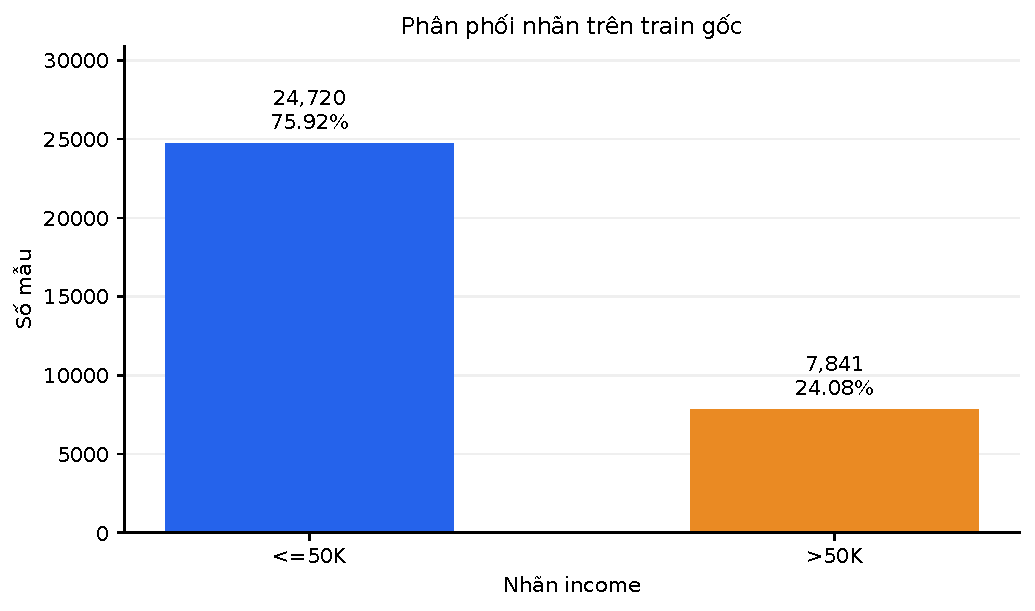
\includegraphics[width=.92\textwidth,height=.72\textheight,keepaspectratio]{Images/chapter_3/3_4/label_distribution.pdf}
\caption{Số lượng và tỷ lệ hai nhãn trên adult.data gốc}
\label{fig:label-distribution}
\end{figure}
